\chapter{Introduction to Signed digraph }
In this chapter we study signed digraph and discuss some of its properties.We work throughout with real matrices and begin by introducing some notation and definitions.
\section{Signed digraph}
\begin{dfn}
	Let $A$ be a real matrix of order $n$, its signed digraph $SD(A)$ is a directed graph with nodes labeled from ${1,2,\dots,n}$ and there is a directed edge from node $i$ to node $j$ iff the entry $a_{ji}$ in $A$ is non-zero.\newline
	 If $a_{ji}$ is positive, the edge connecting from node $i$ to node $j$ is labelled with positive sign and if $a_{ji}$ is negative,the edge connecting from node $i$ to node $j$ is labelled with negative sign.
	
\end{dfn}
  The set of all matrices with the same sign pattern (and thus having the same signed digraph) as $A$ is denoted by $Q(A)$. We also use the undirected graph $G(A)$ which has the same node set as $SD(A)$ with edge set $\{\{i,j\}:i\neq j \text{ and }$. An edge of $G(A)$ thus corresponds to a 2-cycle in $SD(A)$.
  
  \begin{example}
  	Consider the matrix given by
  	 \begin{center}
  		$ A =$ 
  	$	\begin{bmatrix}
  			1 & 2 & 0 & 0\\
  			2 & 0 & -3 & 2\\
  			0 & 2 & -1 & 0 \\
  			0 & -1 & 0 & -3
  		\end{bmatrix}$
  	\end{center} 
  
  It's associated signed digraph is given by:
  \begin{center}
  	 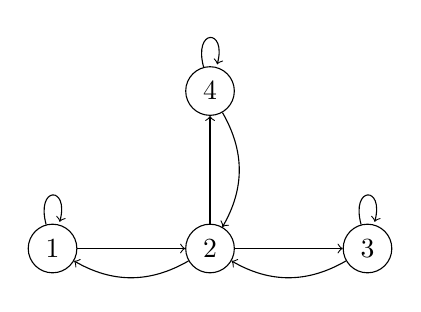
\begin{tikzpicture}
  		% Nodes
  		\node[circle, draw] (1) at (0,0) {1};
  		\node[circle, draw] (2) at (2,0) {2};
  		\node[circle, draw] (3) at (4,0) {3};
  		\node[circle, draw] (4) at (2,2) {4};
  		
  		% Edges
  		\draw[->] (1) -- (2);
  		\draw[->] (1) edge [loop above] ();
  		\draw[->] (2) -- (3);
  		\draw[->] (2) -- (4);
  		\draw[->] (3) edge [loop above] ();
  		%	\draw[->] (4) -- (2);
  		\draw[->] (4) edge [loop above] ();
  		
  		% Separate directed edges from 2 to 1 and 1 to 2
  		\draw[->] (2) to [bend left] (1);
  		\draw[->] (3) to [bend left] (2);
  		\draw[->] (4) to [bend left] (2);
  	\end{tikzpicture}
  \end{center}

  
  \end{example}

  
  \begin{dfn}
  	A 2-cycle in $SD(A)$ is positive if $a_{ij}a_{ji} > 0$ and negative if $a_{ij}a_{ji} < 0$
  \end{dfn}
   
   \begin{example}
   	 In the above matrix \( A \), \( a_{12} \cdot a_{21} > 0 \), indicating a positive 2-cycle in the signed digraph \( SD(A) \). Conversely, \( a_{23} \cdot a_{32} < 0 \), indicating the presence of a negative 2-cycle in \( SD(A) \).
   \end{example}

  \begin{dfn}
   	A node $i$ with a 1-cycle is called distinguished and it corresponds to a nonzero diagonal entry in $A$,i.e, $a_{ii} \neq 0$.
  \end{dfn}

   \begin{example}
   	 In the above matrix $A$, node 1,3,4 are distinguished nodes and corresponds to non-zero diagonal entry. 
   \end{example}

	Let's consider the differential equation $\dot{x}(t) = Ax(t)$ with $A \in Q(A)$, and we are going to detect the possibility of constant or sinusoidal trajectories.

   \begin{dfn}
   	A constant (strictly constant) trajectory $x(t) \in \mathbb{R}^n$ for $\dot{x}_i = \sum_{j=1}^n a_{ij}x_j$ satisfies $\dot{x}_i = 0$ and $x_i \neq 0$ for some (all) $i$
   	\end{dfn}
   
   \begin{dfn}
   	A sinusoidal (strictly sinusoidal) trajectory for our equation satisfies $\ddot{x}_i = -x_i$ and $x_i \not\equiv 0$ ("not the constant function with the value zero") for some (all) $i$.
   	\end{dfn}
   
   \begin{lem}
      Consider the differential equation $\dot{x} = \tilde{A}x$. Then it admits a constant (sinusoidal) trajectory if and only if $\tilde{A}$ has a zero (purely imaginary) eigenvalue.
   \end{lem}
 

 \section{$\lambda$-consistency}
 \begin{dfn}
 	Suppose $G(A)$ is a tree. A signed digraph $SD(A)$ is said to be $\lambda$-consistent if there exist nonzero constants $\{\lambda_1, \ldots, \lambda_n\}$ such that $\lambda_i a_{ij} = -\lambda_j a_{ji}$ for $i \neq j$; all $\lambda_ia_{ii} > 0$; and some $\lambda_ia_{ii} > 0$.
 	\end{dfn}

  %For example, matrices with $a_{ij}a_{ji} < 0$ for all $i\neq j$, $a_{ii} \leq 0$ for all $i$, and $a_{ii} < 0$ for at least one $i$ have $SD(A)$ $\lambda$-consistent with all $\lambda_i$ negative. These matrices are candidates for sign stability [4].
   \subsection*{How to find whether a matrix is $\lambda$-consistent?}
	
	Consider a case where node 1 is a distinguished node in the \( \lambda \)-consistent \( SD(A) \), having \( a_{11} \neq 0 \). Let's select \( \lambda_1 = \pm 1 \), ensuring \( \lambda_1 a_{11} > 0 \). Using the signs of 2-cycles along the chain, we can determine the signs of all other \( \{\lambda_j\} \) values.This process can be done because due to the tree structure of $G(A)$.\textbf{Consequently, \( SD(A) \) exhibits \( \lambda \)-consistency if and only if each \( \lambda_i a_{ij} > 0 \).} 
	

\begin{example}
		Consider the matrix given by
	\begin{center}
		$ A =$ 
		$	\begin{bmatrix}
			1 & 2 & 0 & 0\\
			2 & 0 & -3 & 2\\
			0 & 2 & -1 & 0 \\
			0 & -1 & 0 & -3
		\end{bmatrix}$
	\end{center} 

   In this analysis, node 1 is identified as a distinguished node where $a_{11} > 0$. Consequently, we choose $\lambda_1$ such that $\lambda_1 a_{11} > 0$, leading us to set $\lambda_1 = 1$, which indicates a positive value.
   
   The signs of the remaining $\lambda_j$ values are determined using the properties of 2-cycles:
   \begin{enumerate}
   	\item The relationship $\lambda_1 a_{12} = -\lambda_2 a_{21}$, with both $a_{12}$ and $a_{21}$ equal to 2 and positive, implies that $\lambda_2 = -1$, which is negative.
   	\item Considering $\lambda_2 a_{23} = -\lambda_3 a_{32}$ where $a_{23} = -3$ (negative) and $a_{32} = 2$ (positive), we find $\lambda_3 = -\frac{3}{2}$, also negative.
   	\item For the cycle involving nodes 2 and 4, $\lambda_2 a_{24} = -\lambda_4 a_{42}$, with $a_{24} = 2$ (positive) and $a_{42} = -1$ (negative), leads us to conclude $\lambda_4 = -2$, again negative.
   \end{enumerate}
   
   Finally, we validate the diagonal entries for $\lambda$-consistency, ensuring that $\lambda_i a_{ii} > 0$ holds for all nodes $i \in \{1, 2, 3, 4\}$.
   
   Therefore, the matrix $A$ is confirmed to be $\lambda$-consistent, based on these considerations.
   
   
\end{example}

 \begin{example}
 		Consider the matrix given by:
 	\begin{center}
 		$ B =$ 
 		$	\begin{bmatrix}
 			-1 & 2 & 0 & 0\\
 			3 & 1 & 1 & 0\\
 			0 & -2 & 0 & -4 \\
 			0 & 0 & 2 & -1
 		\end{bmatrix}$
 	\end{center} 
	  In this analysis, node 1 is identified as a distinguished node where $a_{11} = -1$, which is less than zero. Therefore, we select $\lambda_1$ such that $\lambda_1 a_{11} > 0$. This requirement implies that $\lambda_1 = -1$, which is negative.
	  
	  Next, we determine the signs of the remaining $\lambda_j$ values using the properties of 2-cycles:
	  \begin{itemize}
	  	\item For the cycle involving nodes 1 and 2, the relationship $\lambda_1 a_{12} = -\lambda_2 a_{21}$, where $a_{12} = 2$ (positive) and $a_{21} = 3$ (positive), implies $\lambda_2 = -\frac{2}{3}$, which is negative.
	  	\item Similarly, considering $\lambda_2 a_{23} = -\lambda_3 a_{32}$ with $a_{23} = 1$ (positive) and $a_{32} = -2$ (negative), results in $\lambda_3 = -\frac{1}{3}$, also negative.
	  	\item For the cycle involving nodes 2 and 4, $\lambda_2 a_{34} = -\lambda_4 a_{43}$, where $a_{34} = -4$ (negative) and $a_{43} = 2$ (positive), leads to $\lambda_4 = -2$, again negative.
	  \end{itemize}
	  
	  Finally, we check the diagonal entries to verify $\lambda$-consistency. We ensure that $\lambda_i a_{ii} > 0$ for all nodes $i \in \{1, 3, 4\}$. However, node 2 is an exception in this consistency check.
	  
	  Consequently, matrix $B$ is not $\lambda$-consistent.
	  
 
 \end{example}

\begin{dfn}
	A subchain of the signed digraph $SD(A)$ is a subgraph that consists of a sequence of nodes connected by directed edges, forming a straight chain of 2-cycles. Consequently, the undirected graph representing this subchain forms a simple path  (that is, an unbranched tree)
	
\end{dfn}

\begin{lem}
	  When $SD(A)$ has at least two 1-cycles, then $SD(A)$ is not $\lambda$-consistent iff some subchain of $SD(A)$ with distinguished end nodes and no other distinguished nodes, is not $\lambda$-consistent.
\end{lem}

\begin{dfn}
	A subchain in a signed digraph $SD(A)$ such that it has distinguished end nodes and no other distinguished nodes is called \textbf{proper subchain}.
\end{dfn}

\begin{example}
		Consider the matrix given by
	\begin{center}
		$ C =$ 
		$	\begin{bmatrix}
			1 & 2 & 0 & 0\\
			2 & 0 & -3 & 2\\
			0 & 2 &  1 & 0 \\
			0 & -1 & 0 & 3
		\end{bmatrix}$
	\end{center} 
  In this case, node 1 is identified as a distinguished node with \(a_{11} = 1 > 0\). Consequently, we choose \(\lambda_1\) such that \(\lambda_1 a_{11} > 0\). This condition dictates that \(\lambda_1 = 1\), which is positive.
  
  To determine the signs of the remaining \(\lambda_j\) values, we examine the information from the 2-cycles:
  \begin{itemize}
  	\item Considering the cycle between nodes 1 and 2, the relationship \(\lambda_1 a_{12} = -\lambda_2 a_{21}\) holds, where \(a_{12} = 2\) and \(a_{21} = 2\), both positive. This leads to \(\lambda_2 = -1\), which is negative.
  	\item Analyzing the cycle between nodes 2 and 3, where \(\lambda_2 a_{23} = -\lambda_3 a_{32}\), with \(a_{23} = -3\) (negative) and \(a_{32} = 2\) (positive), it follows that \(\lambda_3 = -\frac{3}{2}\), also negative.
  	\item For the cycle involving nodes 2 and 4, given \(\lambda_2 a_{24} = -\lambda_4 a_{42}\), with \(a_{24} = 2\) (positive) and \(a_{42} = -1\) (negative), it implies that \(\lambda_4 = -2\), which is negative.
  \end{itemize}
  
  We then verify the diagonal entries for \(\lambda\)-consistency. Therefore, \(\lambda_i a_{ii} > 0\) for \(i \in \{1, 2\}\), but not for nodes 3 and 4.
  
  Hence, matrix C is not \(\lambda\)-consistent.
  
  
\end{example}

Verifying the above mentioned lemma is straightforward, as we identify a proper subchain with the node set \(\{1, 2, 3\}\) featuring distinguished end nodes. This subchain is not \(\lambda\)-consistent, thereby confirming that matrix C is also not \(\lambda\)-consistent.
 


